%%%%%%%%%%%%%%%%%%%%%%%%%%%%%%%%%%%%%%%%%%%%%%%%%%%%%%%%%%%%%%%%%%%%%
%%                                                                 							%%
%%		Trabajo Fin de GRADO		                       				%%
%%		TITULO 																			%%
%%		AUTOR												%%
%%                                                                 							%%
%%%%%%%%%%%%%%%%%%%%%%%%%%%%%%%%%%%%%%%%%%%%%%%%%%%%%%%%%%%%%%%%%%%%%

%%  Include con la definicion de estilos por el usuario
%%%%%%%%%%%%%%%%%%%%%%%%%%%%%%%%%%%%%%%%%%%%%%%%%%%%%%%%%%%%%%%%%%%%%

\input definl

%%  Paqueteria necesaria de fabrica
%%%%%%%%%%%%%%%%%%%%%%%%%%%%%%%%%%%%%%%%%%%%%%%%%%%%%%%%%%%%%%%%%%%%%
\usepackage{hyperref}
\usepackage{palatino}
\usepackage[dvips]{graphicx} 	  % para importar combinados latex
\usepackage{color}          		      % para importar dibujos coloreados
\usepackage{rotating}        		  % para usar \begin{sideways} que rota tabla 90 grados 
\usepackage{epsfig}          		  % para rotar figuras de Xfig  poniendo % \begin{sideways} 
\usepackage{amsmath}         	  % para usar matrix y pmatrix environment
\usepackage{stmaryrd}        		  % para usar la \bigsqcap
\usepackage{verbatim}        		  % para poner salidas de pantallas
\usepackage{listings}       	 	  % para imprimir codigo fuente
\usepackage{shortvrb}				  % 
\usepackage{url}						  % 
\usepackage{subfigure}			  % 

  

%%%%%%%%%%%%%%%%%%%%%%%%%%%%%%%%%%%%%%%%%%%%%%%%%%%%%%%%%%%%%%%%%%%%%
%%  Configuracion de paquetes
%%%%%%%%%%%%%%%%%%%%%%%%%%%%%%%%%%%%%%%%%%%%%%%%%%%%%%%%%%%%%%%%%%%%%
\renewcommand\lstlistingname{Listado}                   %  default is Listing
%\renewcommand\lstlistlistingname{\'Indice de listados}  %  default is Listings 
%\renewcommand\thelstlisting{\thechapter .\arabic{lstlisting}} % captionstyle


\lstset{
  language=Java,
  basicstyle=\small,
  keywordstyle=\bfseries,
  showstringspaces=false,
  numbers=left, 
  numberstyle=\tiny, 
  stepnumber=1, 
  numbersep=5pt,
  frame=single}


%%  Configuraciones varias
%%%%%%%%%%%%%%%%%%%%%%%%%%%%%%%%%%%%%%%%%%%%%%%%%%%%%%%%%%%%%%%%%%%%%
\newcommand{\corregir}{\color{blue}}  	 	% pintar en color azul
\setlength{\parskip}{2ex}              			% despues del parrafo, doble linea


% Para que no aparezcan las cabeceras de las páginas que están en blanco
%%%%%%%%%%%%%%%%%%%%%%%%%%%%%%%%%%%%%%%%%%%%%%%%%%%%%%%%%%%%%%%%%%%%%
\makeatletter 
\def\cleardoublepage{\clearpage\if@twoside \ifodd\c@page\else
  \hbox{} 
  \thispagestyle{empty} 
  \newpage
  \if@twocolumn\hbox{}\newpage\fi\fi\fi} 
\makeatother

%%  Cortes de palabras especiales
%%%%%%%%%%%%%%%%%%%%%%%%%%%%%%%%%%%%%%%%%%%%%%%%%%%%%%%%%%%%%%%%%%%%%
\hyphenation{
ejem-plo Algo-ritmo
}


%\includeonly{titulo, prologo,intro,capitulo1}


\begin{document} 

%%  Titulo e Indices
%%%%%%%%%%%%%%%%%%%%%%%%%%%%%%%%%%%%%%%%%%%%%%%%%%%%%%%%%%%%%%%%%%%%%%
\pagenumbering{roman}
\thispagestyle{empty}

{


\thispagestyle{empty}
\begin{center}

\includegraphics[scale=.6]{img/logous}
\end{center}

\vspace*{0cm}
\Large 

\begin{center}

{\normalsize \sc Escuelta Técnica Superior de Ingeniería Informática}

{\large \bf Máster Oficial en Lógica, Computación e\\ Inteligencia Artificial }

\vspace*{1.5cm}

{\sc Trabajo Fin de Máster}


{\LARGE \bf Conciliación de Conceptos Formales \\ en Sistemas de Etiquetado\\ mediante Sistemas MultiAgente}

\end{center} 




\vspace*{0.5cm}
%\vfill

\begin{center}
{\normalsize Autor: \\ {\bf Jesús Giráldez Crú}}
\end{center}

\begin{center}
%{\footnotesize Tutores:}
{\small Tutores: }
\vspace*{0.2cm}
{\small \\  Joaquín Borrego Díaz \\ Gonzalo A. Aranda Corral}
\end{center}

\vspace*{0.5cm}
\vfill
\begin{center}
{\footnotesize Sevilla, 30 de junio de 2011.\\Curso académico 2010/11. Primera Convocatoria}
\end{center}

%
%\hspace*{.5\textwidth}
%\normalsize
%\begin{tabular}{l}
%
%Trabajo Fin de Máster\\
%de Jesús Giráldez Crú \\
%dentro del programa de Máster en \\
%Lógica, Computación 
%e Inteligencia Artificial\\
%
%% para optar al grado de \\
%% 
%% trabajo de investigaciÛn\\
%% 
%% por la Universidad de Sevilla \\
%%  
%\end{tabular} \par
%
%% \vspace{2cm}
%% 
%% \hspace*{.5\textwidth}  
%% \quad Gonzalo Antonio Aranda Corral \par
%% 
%
%\vspace*{-2.9cm}
%
%V. B. Director
%
%\vspace*{4cm}





\newpage
\thispagestyle{empty}
\mbox{ }
\newpage
\thispagestyle{empty}

\newpage
\thispagestyle{empty}

\mbox{ }

\vfill

\begin{flushright}
  \begin{minipage}{9cm}
%\begin{right}
%    \em{``El hombre es inteligente porque tiene manos''}\\ \\Anax·goras 
%\end{right}
%    \em{``Iré a cualquier parte, siempre que sea hacia delante.''}\\ \\ 
%David Livingston.


%{\em Ya veré...}

\end{minipage}
\end{flushright}

\vfill

\newpage
\thispagestyle{empty}
\mbox{ }

}

%! \newpage
%! \chapter*{Agradecimientos}
%! \thispagestyle{empty}
%! 
%! Agradecimientos a todo el personal
%! 
%! \newpage
%! \thispagestyle{empty}
%! \mbox{ }
%! 
%%% Local Variables: 
%%% mode: latex
%%% TeX-master: "../dea"
%%% End: 
  

\clearpage
\pagestyle{plain}
\tableofcontents
\clearpage
\listoffigures

%%  Contenido del trabajo
%%%%%%%%%%%%%%%%%%%%%%%%%%%%%%%%%%%%%%%%%%%%%%%%%%%%%%%%%%%%%%%%%%%%%%
\pagenumbering{arabic}
\pagestyle{fancy}

%\chapter*{Prólogo}
\label{intro:prologo}
\addcontentsline{toc}{chapter}{Prólogo}

	La conciliación es...
\chapter*{Introducción}
\label{intro:intro}
\addcontentsline{toc}{chapter}{Introducción.}

En ocasiones, la búsqueda de información sobre ciertos temas en Internet se convierte en una ardua tarea, debido a que los resultados que encontramos no son demasiado relevantes. Esto se debe a numerosas razones. En general, se puede decir que los parámetros con los que ajustamos la búsqueda no termina de ser los más apropiados para conseguir los resultados que esperamos; bien porque no hemos sabido ajustar correctamente las palabras claves en nuestra búsqueda, y por tanto, los resultados obtenidos versan sobre otros temas distintos; o bien porque, aunque estas palabras claves sí sean relativamente correctas, los resultados obtenidos son más específicos o más generales de lo que buscamos, y por tanto estos resultados tampoco son conveniententes. Desde el punto de vista de búsquedas en contextos \emph{semantizados} \footnote{Se entiende por contextos \emph{semantizados} a aquellos que están marcados con ciertos metadatos semánticos.}, podemos decir más concretamente que si los resultados encontrados no son apropiados, es porque el conocimiento con el que hemos ajustado la búsqueda es incompleto, o incluso incorrecto.

Una posible solución para solventar, o minimizar este problema, podría ser el uso del conocimiento de otros usuarios, además del conocimiento propio del usuario, que ya se dispone. De esta forma, una búsqueda podría ser más completa, ya que el usuario no es el único que aporta conocimiento a los parámetros de dicha búsqueda, sino que éstos se enriquecen con el conocimiento de otros usuarios. Por tanto, el problema se traslada a encontrar relaciones entre usuarios y elegir qué conocimiento será usado para complementar el conocimiento propio de cada usuario.

En este trabajo se propone una solución formal a este problema, en el que se intenta complementar los diferentes conocimientos de cada usuario mediante implicaciones lógicas, que permitan establecer una serie de reglas entre ellos. El conocimiento común que genera un par de usuarios es lo que llamamos {\bf Conciliación de Conocimiento}, como se cita en \cite{algoritmo}. Con este conocimiento conciliado se dispone de una herramienta que puede enriquecer semánticamente cualquier búsqueda. Igualmente, es interesante concebir este conocimiento conciliado desde el punto de vista de la navegación entre usuarios, o entre la información de los mismos, que es, al fin y al cabo, otra forma de buscar información en Internet. Este conocimiento conciliado entre dos usuarios representa un conocimiento aceptado por ambos, ya que está basado en implicaciones lógicas, que aportan un trasfondo formal a este conocimiento. Por tanto, este conocimiento conciliado es equivalente a un contexto común entre ambos usuarios. La navegación semántica entre estos usuarios pasa por un punto intermedio, que es precisamente este conocimiento conciliado.

En este trabajo se propone un método de conciliación del conocimiento en sistemas multiusuario, centrando el caso de estudio en los sistemas de etiquetado. Este método se basa en la utilización de cálculos basados en Análisis Formal de Conceptos (se utilizarán técnicas descritas en \cite{afc}), y ha sido implementado en una estructura de Sistema MultiAgente (SMA) en una plataforma JADE (consutar \cite{jade}).




\section*{Internet, Datos e Información.}
\addcontentsline{toc}{section}{Internet, Datos e Información}

Hoy en día, Internet se ha convertido en una herramienta básica en nuestro día a día. La generación de contenido se produce de una forma masiva, y el volumen de contenido generado crece en forma exponencial; es decir, en cada momento, en Internet se genera una cantidad de contenido mucho mayor que el contenido que se ha generado previamente. Este crecimiento exponencial de Internet es una realidad, y existen algunos problemas que derivan de él, como la gestión de esa cantidad tan grande de contenido.

En los últimos tiempos, este crecimiento del contenido se ha potenciado debido al crecimiento de la Web 2.0, que aporta potentes tecnologías para compartir este contenido con el resto de usuarios (ver \cite{algoritmo} y \cite{mowento}). Ejemplo de ello, es el gran número de herramientas sociales (redes sociales, sistemas de etiquetado, sistemas de compartición de ficheros, etc.), en los que se establece cierta conexión entre los usuarios, y en los que, cada vez más, se integran contenidos multimedia junto con el formato de texto plano que siempre ha existido. El hecho de que estos contenidos multimedia se conviertan en uno de los pilares básicos de esta Web 2.0, trae consigo ciertas consecuencias:

\begin{itemize}
	\item La generación de contenido se vuelve cada vez más masiva, debido al hecho de que el contenido multimedia es más amigable para el usuario. Los avances tecnológicos han propiciado este hecho, debido a que las fronteras de Internet llegan cada vez a más usuarios, y las velocidades de acceso a éste son cada vez más rápidas, y esto hace viable esta generación tan masiva de este contenido, así como su visualización posterior.
	\item El contenido multimedia es, si cabe, más difícil de gestionar y procesar que cualquier contenido en texto plano. Por una parte, el texto plano responde a unos formatos más restringidos, por lo que se podría considerar casi estándar. Sin embargo, el contenido multimedia se clasifica en diferentes tipos (audio, vídeo, imágenes, etc.), en los que cada tipo se clasifica en numerosos formatos. Por tanto, las tareas de gestión son bastante más complicadas, puesto que hay que enfrentarse a diferentes tareas en función del tipo de contenido y del formato del mismo. Por otra parte, el procesado de este contenido también es más complicado. Una búsqueda en un texto plano es, a grosso modo, una tarea de coincidencia de cierta secuencia de caracteres; aunque hoy en día, estas tareas son mucho más complejas que esa simple idea. Sin embargo, en cualquier caso, es una tarea con un coste computacional bajo, y por tanto, rápida. En cambio, en el ámbito del contenido multimedia esta tarea es mucho más complicada. Un símil equivalente podría ser buscar cierta forma en una imágen, cierto sonido en un audio o cierto fotograma en un vídeo. Estos ejemplos son casos de estudio actualmente, y la carga computacional de ellos es de un orden muy superior que el ejemplo de búsqueda en texto plano. En conclusión, el procesado de este contenido es más complicado.
\end{itemize}

Otra característica de estas herramientas 2.0 es la posibilidad de relación social que la propia herramienta ofrece al usuario para que se relacione con otros usuarios. Al igual que el crecimiento del contenido, se produce también un crecimiento en cuanto al número de relaciones entre usuarios, que cada vez más, van estableciendo relaciones con otros usuarios, lo que, dependiendo del sistema, permite acceder a su contenido, compartir contenido común, etc.

De una forma abstracta, esta idea puede entenderse como un concepto de grafo, en el que se represente todo este contenido, mediante nodos, y todas estas relaciones entre usuarios, mediante aristas. Por una parte, a medida que se produce un crecimiento en cuanto a la generación de contenido, encontraríamos un crecimiento en el número de nodos del grafo. Por otra, el crecimiento de las relaciones sociales en el ámbito de la Web 2.0, equivale a un crecimiento del número de aristas de este grafo abstracto que representa todo el conjunto de la web (o simplificadamente, representa a un sistema concreto: un sistema de etiquetado concreto, una red social concreta, etc.).

En conclusión, el crecimiento de Internet hoy en día lleva consigo:
\begin{enumerate}
	\item Una generación masiva de contenido, en gran parte multimedia.
	\item Un problema de procesado de este contenido, debido al gran volumen de los mismo. Y un problema asociado al contenido multimedia, debido a la propia naturaleza de este contenido.
	\item Un conjunto de relaciones entre usuarios de gran volumen.
\end{enumerate}

Es obvio que un trabajo de procesamiento o gestión sobre este compendio de contenido es inviable si se realiza a nivel global. En esta línea, hablaremos de {\bf datos} cuando, en casos como el anteriormente descrito, se disponga de una gran cantidad de contenido pero que es difícil de procesar, analizar y tratar. Sin embargo, es posible añadir cierta metainformación sobre estos datos, para conseguir que estas tareas se puedan llevar a cabo con relativa viabilidad. Con esta metainformación, todo el contenido se puede clasificar más fácilmente, y esta clasificación posibilita un procesado posterior a nivel global que sea viable en cuanto a tiempos de ejecución o carga computacional. Esta metainformación será, en su mayoría, ciertos metadatos semánticos que se añadan a los datos. En el caso de contenido marcados semánticamente, hablaremos de {\bf información}.






\section*{Motivación y Objetivos.}
\addcontentsline{toc}{section}{Motivación y Objetivos}

En la sección anterior, se introduce la posibilidad del marcado semántico (mediante metadatos añadidos al contenido), para convertir los \emph{datos} en \emph{información}. Una vez hecho esto, las posibilidades de procesado a posteriori de esta información son innumerables.

En este trabajo se propone el uso de los Sistemas de Etiquetado, en los que encontramos información marcada semánticamente, con etiquetas, como se verá en el capítulo~\ref{cap:capitulo3}; para llevar a cabo un procesado semántico con el que obtener un conocimiento conciliado entre varios usuarios. Inicialmente se propone conseguir este conocimiento conciliado por pares de usuarios que formen parte del sistema, si bien, en un futuro se puede ampliar a un concepto superior de conocimiento conciliado global. La principal motivación de este trabajo es encontrar un método de conciliación que sea aplicable a sistemas de etiquetado de este tipo, aunque en un futuro se podría ampliar a otro tipo de sistemas. Estas conciliaciones representan un método de navegación entre usuarios, puesto que el conocimiento conciliado que se obtenga para cada par de usuarios, representará un conocimiento común que ambos usuarios aceptan, y por tanto, puede ser una herramienta útil de navegación entre ellos. En un futuro, este conocimiento conciliado podría ser usado en otras tareas como refinamientos de búsquedas, depuración semántica, etc.

Los principales objetivos de este trabajo son:

\begin{itemize}
	\item Formalizar el conocimiento de los Sistemas de Etiquetado.
	\item Extraer los distintos elementos de AFC de estos sistemas.
	\item Implantar un método de conciliación a escala global para todo el conjunto de alguno de estos sistemas.
	\item Analizar los resultados y proponer soluciones futuras que aporten una funcionalidad clara y útil a estos sistemas.
\end{itemize}





\section*{Solución Propuesta.}
\addcontentsline{toc}{section}{Solución Propuesta}

La solución propuesta es un Sistema MultiAgente (SMA) implementado en JADE (ver \cite{jade}), en el que se extraiga el conocimiento de un caso práctico concreto, y calcule un conocimiento conciliado para este sistema. El caso práctico concreto que utilizaremos será un subconjunto de datos de Delicious (ver \cite{delicious}). En el SMA, un conjunto de agentes, que representan a los usuarios del sistema, negociarán entre ellos para conciliar su conocimiento con otros usuarios, en función de su disponibilidad y de la prioridad que tengan en realizar otras conciliaciones con terceros. A medida que avance la ejecución del SMA, se irán produciendo múltiples conciliaciones de forma paralela, de forma que el conocimiento conciliado sea cada vez mayor; y por tanto, se enriquecerá este conocimiento común. Este conocimiento conciliado será almacenado, de forma que se puedan realizar cálculos o extraer conclusiones posteriormente.

En el capítulo~\ref{cap:capitulo6} se comenta la estructura, componentes y funcionamientos de este SMA. En los capítulos anteriores se comentarán algunas técnicas y herramientas necesarias para llevarlo a cabo, o ciertas formalizaciones previas que justifican el trasfondo formal de este trabajo.






\section*{Estructura de la memoria.}
\addcontentsline{toc}{section}{Estructura de la memoria}

Esta memoria se estructura en varios capítulos, con la siguiente distribución de los temas trabajados:

\begin{itemize}
	\item Capítulo~\ref{cap:capitulo1}. Se presenta el Estado del arte en el que se detalla los diferentes modelos de clasificación de la información en Internet, y se plantean las diferentes problemáticas de cada uno de estos modelos.
	\item Capítulo~\ref{cap:capitulo2}. Se formalizan las nociones mátematicas de Análisis Formal de Conceptos (AFC) que sirven como soporte formal en este trabajo.
	\item Capítulo~\ref{cap:capitulo3}. Se introducen los Sistemas de Etiquetado, que serán los casos de estudio concretos de este trabajo, viendo su estructura y la extracción formal de los conceptos de AFC vistos en el capítulo anterior.
	\item Capítulo~\ref{cap:capitulo4}. Se explica el Algoritmo de Conciliación, que permite conciliar el conocimiento de un par de usuarios.
	\item Capítulo~\ref{cap:capitulo5}. Se describen las características del Conjunto de Datos con el que llevaremos a cabo los procesos de prueba empíricamente.
	\item Capítulo~\ref{cap:capitulo6}. Se explica el Sistema MultiAgente (SMA) que se plantea como solución en este trabajo: comportamiento, estructura y componenentes.
	\item Capítulo~\ref{cap:capitulo7}. Se detallan los resultados obtenidos en una prueba empírica llevada a cabo, y se analizan estos resultados.
	\item Capítulo~\ref{cap:capitulo8}. Finalmente, se comentan las conclusiones obtenidas, así como los puntos de trabajo futuro.
	\item Bibliografía.
\end{itemize}
\chapter{Estado del Arte.}\label{cap:capitulo1}

En este capítulo, se introducirá de forma general el estado del arte sobre la clasificación de los datos y la información en Internet, se introducirán los Sistemas de Etiquetado como herramienta de marcación semántica de ciertos datos, se tratarán los diferentes problemas asociados a esta marcación semántica, y finalmente se introducirá la Conciliación de Conceptos como método formal para encontrar conocimiento común entre usuarios.


\section{Clasificación del contenido en Internet.}

La organización del contenido en Internet se realiza a menudo a través de marcas en el contenido con términos descriptivos, también llamados \emph{palabras clave} o \emph{etiquetas}. Esta organización permite al usuario ciertas tareas futuras como navegación, filtro o búsquedas. Esta forma de organización no es, ni mucho menos, nueva; sin embargo, sus creadores en el ámbito de Internet, le acuñaron el nombre de {\bf etiquetado}, con el que actualmente se conoce, y que está ganando mucha popularidad en Internet.

Históricamente, la asignación de estas palabras claves para la organización de colecciones o librerías ha sido tarea de una persona experta en la materia que, bajo su criterio, es quién elige el conjunto de palabras clave y la asignación de las mismas a los diferentes recursos, como se explica en \cite{rowley}. En cambio, el etiquetado colaborativo permite que cualquier usuario participe en esta tarea, de forma que cada recurso pueda ser etiquetado con palabras claves por cualquier usuario y por cualquier palabra clave que éstos elijan.

En cuanto a sistemas de clasificación de contenido, se van a distiguir dos tipos: taxonomías y folksonomías.

Las taxonomías son sistemas de clasificación de contenido basados en la categorización de los recursos (o de los elementos, en general). Esta definición se puede entontrar en \cite{smith}, \cite{kim} o \cite{golder}. Estas categorías deben formar un conjunto completo\footnote{Entiéndase \emph{completo} para un ámbito concreto.} y disjunto; de forma que todos los recursos tengan una categoría con la que pueda ser categorizado, y que además, se elimine (o en todo caso, se minimice) las posibles ambigüedades entre varias categorías. La única excepción en este conjunto disjunto se produce debido a la posibilidad de establecer una jerarquía en las categorías, de forma que se establezca una especialización de las mismas. Estos sistemas son, por tanto, jerárquicos y exclusivos. 

En la otra cara de la moneda, encontramos otros sistemas no jerárquicos y no exclusivos: las folksonomías, cuya definición está aproximadamente consensuada. Esta definición se puede consultar en  \cite{smith}, \cite{kim}, \cite{golder}, \cite{gruber} o \cite{knerr}. En este tipo de clasificación, cada recurso es marcado con una serie de etiquetas, que aportan a estos recursos una serie de metadatos semánticos. En \cite{smith}, se comentan los distintos sistemas que incorporan folksonomías como herramientas; y se discute las diferentes restricciones de cada uno de ellos: conjunto de etiquetas restringido o abierto, etiquetación a recursos propios o globales del sistema, etc. En \cite{golder}, se explica la diferencia entre estos sistemas y los anteriores, cuya principal diferencia es la opción de trabajar con interesecciones entre las diferentes categorías que aparecen, consiguiendo una mejor organización de los recursos y evitando posibles duplicidades de los mismos.

Esta diferencia hace que estos sistemas de etiquetado se hayan convertido en una herramienta muy útil en gran cantidad de sistemas que funcionan en Internet, gracias a la versatilidad que ofrecen al usuario, y además, al ser una herramienta colaborativa, se gestiona gracias a las aportaciones de todos los usuarios, sin necesidad de que una persona experta se encargue de esta tarea. Prueba del auge de estas herramientas, es el enorme número de trabajos que hay sobre ellos desde diversos puntos de vista, como el análisis (estadístico) de los modelos de etiquetación realizado en \cite{golder}, la recuperación y navegación por la información realizado en \cite{halpin} o \cite{jaschke}, o el análisis de redes sociales realizado en \cite{mika} o \cite{brooks}.


\section{El Etiquetado y la Web Semántica.}

Como se ha comentado en la sección anterior, las folksonomías dotan a cualquier sistema en el que se implanten, de una herramienta colaborativa con la cual organizar el contenido. Además, debido a sus características no jerárquicas y no exclusivas, se evitan problemas derivados de otro tipo de clasificaciones, como las taxonomías. Por último, el carácter colaborativo de estas folksonomías han potenciado su popularidad en la Web 2.0, dónde el usuario es el protagonista y \emph{creador} de la propia web (redes sociales, blogs, sistemas de etiquetado, sistemas para compartir ficheros multimedia, etc.).

Por otra parte, estas folksonomías ofrecen una buena alternativa a la web semántica o las ontologías, como se explica en \cite{golder}. Es cierto que estas opciones generan una mayor cantidad de información semántica referente a los recursos del sistema. En cambio, los sistemas de etiquetado, como las folksonomías generan una información semántica muy pobre, que además es ambigua, como se comenta en \cite{algoritmo} y \cite{golder}; en comparación con un sistema basado en ontologías, por ejemplo. En éste último, el marcado semántico es completo, y el procesado semántico (que es la motivación de este trabajo), sería más fácil.

Sin embargo, el concepto de web semántica puede chocar en algunos aspectos con el carácter colaborativo propio de estas folksonomías de los sistemas de etiquetado. Precisamente, uno de los puntos más enriquecedores de estos sistemas es que la información semántica la generan los usuarios, para ser procesada y/o gestionada por ellos mismos. Si bien no existe una formalización en cuanto a la semantización de la información, el papel que juegan los usuarios es crucial para haber conseguido un desarrollo tran grande (frente a otros sistemas, basados en ontologías por ejemplo, que son propios de otro tipo de casos de estudio).

En cambio, como se introdujo en el capítulo anterior, es necesario cierto procesado de la información, para obtener un mecanismo que formalice la semántica de estos sistemas. Las etiquetas serán los elementos que proporcionen esta formalización.






\section{Sistemas de Etiquetado.}

En \cite{smith}, se tratan diversos Sistemas de Etiquetado y las diferentes características de cada una de sus arquitecturas.

De forma general, diremos que un Sistema de Etiquetado está compuesto por Recursos, Etiquetas y Usuarios. En nuestro caso de estudio, los recursos estarán disponibles para cualquier usuario, de forma que un recurso pueda estar etiquetado por múltiples usuarios. El conjunto de recursos es abierto; es decir, cualquier usuario puede añadir nuevos recursos al sistema, por lo que este conjunto está continuamente creciendo. Igualmente ocurre en el caso del conjunto de etiquetas, de forma que una etiqueta puede ser usada por múltiples usuarios, y cada usuario puede añadir las etiquetas que desee al sistema.

En el capítulo~\ref{cap:capitulo3}, se verá de forma detallada las características de los Sistemas de Etiquetado que se tratan en este trabajo. El sistema elegido ha sido Delicious (ver \cite{delicious}), dónde los recursos son URLs que los usuarios guardan, y las etiquetas son campos de texto plano. De esta forma, una URL puede haber sido introducida en el sistema por dos usuarios distintos, por lo que este recurso es \emph{compartido} para ambos (aunque tengan etiquetas distintas para cada uno de ellos). De igual forma, dos usuarios pueden tener etiquetas comunes (o no), que hayan introducido en el sistema.




\section{El Problema de la Heterogeneidad.}

El Etiquetado lleva consigo un problema implícito: la heterogeneidad semántica. En \cite{golder} se comentan algunos aspectos semánticos y cognitivos sobre el proceso de clasificación. Básicamente, se establecen tres problemas principales: polisemia, sinonimia y variaciones del nivel básico.

La polisemia es el problema que se produce debido a que a una palabra tiene varios significados. Al realizar una búsqueda sobre este término, un sistema no sería capaz de distinguir estos significados diferentes; y por tanto, se obtienen más resultados de los esperados, ya que muchos de ellos pertenecen a alguno de los otros significados del término. Esto deriva en un problema de incorrección, pues se obtienen resultados que no deberían obtenerse. Además, este problema es equivalente al producido por homonimia (en concreto, por homografía).

La sinonimia es el problema que se produce debido a que diferentes palabras tienen el mismo significado. Al realizar una búsqueda sobre alguno de estos términos, el sistema sólo será capaz de devolver aquellos resultados que coincidan con el término con el que se ha hecho la búsqueda, obviando todos los resultados de los otros términos sinónimos a éste. Esto deriva en un problema de incompletitud, pues no se obtienen todos los resultados esperados. Además de la definición de sinonimia en lingüística, este problema es equivalente a otros problemas derivados de la escritura propia del usuario. Por ejemplo, las etiquetas \emph{gato} y \emph{gatos} son sinónimos en la práctica, al igual que \emph{para-leer} y \emph{para\_leer}.

Finalmente, existe un problema derivado de las variaciones del nivel básico. En \cite{tanaka} se explica que el nivel básico asocia un problema que surge al existir diferentes términos que describen un único objeto en el rango desde lo más general a lo más específico; el nivel básico es precisamente el que se asocia mayormente con las interacciones humanas. Por ejemplo, \emph{animal}, \emph{perro} y \emph{dálmata} corresponde a la misma categoría, desde la más general a la más concreta. En el ejemplo anterior, para la mayoría de la gente, el nivel básico se establecería en el término \emph{perro}. Sin embargo, existen algunas variaciones sistemáticas en lo que cada individuo considera el nivel básico. Y estas variaciones plantearían este problema, cuya principal consecuencia es incompletitud, aunque también incorrección.

No hay que olvidar que el proceso de etiquetado es básicamente un proceso de interpretación, en el que cada usuario categoriza el contenido en función de una serie de parámetros personales que, en algunos casos, no corresponden con los parámetros del resto.

En \cite{algoritmo}, se describen los problemas anteriores de una forma más formal, en el ámbito del campo de trabajo de los sistemas de etiquetado. Así pues, se tiene:
\begin{itemize}
	\item Hetereogeneidad del Conocimiento dependiente del Contexto (CDKH): Es la limitación producida debido a que una misma etiqueta se refiera a diferentes términos.
	\item Ambigüedad Clásica (CA): Es la limitación producida por las ambigüedades heredadas del lenguaje natural y la elección del nivel básico (\cite{tanaka}) por parte de cada usuario.
\end{itemize}

Por una parte, CA no representa un problema crítico, puesto que el propio objeto (la URL) puede ayudar a desambiguar el significado del término. De hecho, una contextualización de las etiquetas en forma de grafo, puede ayudar a distinguir estos diferentes significados. Sin embargo, CDKH está asociado a estructuras de conceptos que los usuarios no representan en el sistema, aunque métodos de FCA pueden extraer, y por tanto, este problema debe ser tratado con más cautela, y corregido con métodos formales.

Finalmente, hay que comentar que el problema de CDKH es debido a la finalidad con la que se use cierta etiqueta. En \cite{golder}, se definen diferentes tipos de etiquetas:
\begin{itemize}
	\item Identificación del tema que trata: los temas que la URL trata. Por ejemplo \emph{programación}.
	\item Identificación de lo que es: lo que es exactamente la URL. Por ejemplo \emph{libro} o \emph{artículo}.
	\item Identificación del propietario o el creador de la URL. Por ejemplo \emph{Shakespeare}.
	\item Refinación de las categorías. En ocasiones, ciertas etiquetas se usan para complementar la etiquetación de las ya existente. Por ejemplo, números.
	\item Identificación de características: adjetivos, que son la opinión del usuario sobre la URL. Por ejemplo \emph{gracioso} o \emph{estúpido}.
	\item AutoReferencia: del propio usuario. Por ejemplo \emph{mi-libro}.
	\item Etiquetas de organización: ciertas etiquetas se pueden usar para agrupar ciertas URL con un fin común. Por ejemplo \emph{para-leer} o \emph{trabajo-pendiente}.
\end{itemize}



\section{El Etiquetado y la Conciliación de Conceptos.}

Como se ha visto a lo largo del capítulo, en este trabajo se han elegido las folksonomías, y más concretamente los sistemas de etiquetado, como sistemas en los que existen un entorno semantizado, debido a la semántica que las etiquetas aportan a cada objeto del sistema. 

Se ha elegido esta forma de clasificar debido a las ventajas que presenta frente a otros métodos, como taxonomías u ontologías. Sin embargo, se ha explicado los problemas asociados de heterogeneidad y ambigüedad de los términos.

Debido a estos problemas, se han elegido métodos basados en Análisis Formal de Conceptos (AFC) para minimizar las consecuencias de estas ambigüedades semánticas, y establecer un marco de trabajo formal con el que realizar las diferentes operaciones.

La Conciliación de Conceptos es el proceso por el cual, aplicando técnicas de AFC, se van a extraer conceptos formales de los sistemas de etiquetado, tarea que se realizará para cada usuario. Estos conceptos formales nos permitirán calcular un conocimiento común entre los usuarios, que podrá ser usado posteriormente en diferentes tareas: navegación (semántica) entre usuario, refinamiento de búsquedas (semánticas), etc...
   % 
\chapter{Análisis Formal de Conceptos.}\label{cap:capitulo2}

En este capítulo se formalizan algunas nociones sobre {\bf Análisis Formal de Conceptos} (AFC), que serán necesarias para comprender algunas de las técnicas que se usan en el trasfondo de este trabajo. Las definiciones básicas en AFC son las de Contexto Formal y Concepto Formal. El adjetivo \emph{formal} se usa simplemente para indicar que existe un trasfondo matemático en ambas definiciones, y por tanto, su significado difiere de aquellos que tienen en el lenguaje natural.

A lo largo de todo el capítulo, se incluirá un ejemplo que ilustre todas las definiciones que se van incluyendo. Se ha escogido un ejemplo de pequeño tamaño, para facilitarle al lector la lectura y comprensión del proceso; así como la representación de los resultados que se van obteniendo. Sin embargo, estas técnicas que var a ser definidas en este capítulo, serán usadas en el desarrollo de este trabajo con muestras de un tamaño mucho mayor; y por tanto, los resultados serán igualmente de mayor tamaño, por lo que será mucho más difícil representarlos gráficamente.

Se recomienda consultar \cite{afc} como recurso bibliográfico, en el que se formaliza las definiciones de \emph{conjunto}, \emph{conjunto ordenado} o \emph{retículos completos}, que utilizaremos a lo largo de todo el capítulo. Además, se incluyen las demostraciones de todos los teoremas aquí presentados.

\section{Contextos Formales.}

\begin{defi}
	Un {\bf Contexto Formal} $\K := (G, M, I)$ está compuesto por dos conjuntos $G$ y $M$ y una relación $I$ entre $G$ y $M$ ($I \subseteq \{G \times{M}\}$). Los elementos de $G$ son los {\bf objetos} (formales) y los elementos de $M$ son los {\bf atributos} (formales) del Contexto. La relación entre un objeto $g\in{G}$ y un atributo $m\in{M}$, se expresa como $(g,m)\in{I}$ (o $gIm$), y se lee como ``el objeto $g$ tiene el atributo $m$".
\end{defi}

En el siguiente ejemplo, se ilustra un pequeño contexto sobre peces (objetos) y los hábitats en los que viven (atributos):

\begin{itemize}
	\item Un conjunto de Objetos $G$, que son los peces que forman parte de este contexto: carpa, escatófagus, sargo, dorada y anguila.
	\item Un conjunto de Atributos $M$, que son las posibles características de los objetos anteriores, y que en este ejemplo expresan los posibles hábitats de los peces (que no tienen porqué ser exclusivos): fluvial, litoral y océano.
	\item Una relación $I$, entre $G$ y $M$, expresada en la tabla~\ref{fig:contexto}.
\end{itemize}

\begin{figure}[h]

\centering
{ 
\begin{tabular}{|l|c|c|c|}
\hline
& Océano & Litoral & Fluvial \\
\hline
Sargo &  X  &  X  &    \\ \hline
Dorada &  X  &  X  &    \\ \hline
Carpa &    &    &  X  \\ \hline
Anguila &  X  &  X  &  X  \\ \hline
Escatófagus &    &  X  &  X  \\ \hline
\end{tabular}
}
\caption{Ejemplo de Contexto Formal
\label{fig:contexto}
}

\end{figure}

Como se ve en el ejemplo anterior, un contexto puede ser expresado fácilmente en una tabla de doble entrada, dónde las filas se corresponden con los objetos, y las columnas con los atributos. La relación entre ambos se expresa marcando las casillas correspondientes, de forma que si la casilla de la fila $g$ y columna $m$ está marcada, significa que el objeto $g$ tiene el atributo $m$; es decir que $(g,m)\in{I}$, (o $gIm$). En caso contrario, la casilla quedará sin marcar.

De esta forma, se ve como un objeto puede tener múltiples atributos, y un atributo puede pertenecer a varios objetos.

Denotaremos $\{...\}_{\cal X}$ a un subconjunto de elementos del conjunto ${\cal X}$; es decir que $\{...\}_G$ es un subconjunto de objetos, y $\{...\}_M$ es un subconjunto de atributos.



\section{Intención y Extensión.}

Se definen los conjuntos $A'$ y $B'$, de Intención y Extensión de un Contexto ${\cal K} := (G,M,I)$, como:

\begin{defi}
Para un contexto ${\cal K} := (G,M,I)$ y un conjunto $A\in{G}$ de objetos, se define la {\bf Intención} como el conjunto $A'$; que es precisamente el conjunto de atributos comunes a los objetos de $A$:
\begin{center}
$A' := \{m\in{M}|\ gIm\ \forall{g\in{A}}\}$
\end{center}
\end{defi}

\begin{defi}
Para un contexto ${\cal K} := (G,M,I)$ y un conjunto $B\in{M}$ de atributos, se define la {\bf Extensión} como el conjunto $B'$; que es precisamente el conjunto de objetos comunes a los atributos de $B$: 
\begin{center}
$B' := \{g\in{G}|\ gIm\ \forall{m\in{B}}\}$
\end{center}
\end{defi}

Veamos algunos ejemplos de estas operaciones sobre nuestro contexto ejemplo (figura~\ref{fig:contexto}) para ilustrar estas operaciones:
\begin{itemize}
	\item (1): $\{\ fluvial,\ oc\acute{e}ano\ \}'_M\ =\ \{\ anguila\ \}_G$
	\item (2): $\{\ carpa,\ sargo\ \}'_G\ =\ \emptyset_M$
	\item (3): $\{\ escat\acute{o}fagus,\ sargo\ \}'_G\ =\ \{\ litoral\ \}_M$
\end{itemize}

El ejemplo (1) es un ejemplo de extensión de atributos, mientras que los ejemplos (2) y (3) son ejemplos de intención de objetos.







\section{Conceptos Formales.}

\begin{defi}
Un {\bf Concepto Formal} de un Contexto ${\cal K}:=(G,M,I)$ es un par $(A,B)$ con $A \subseteq G$, $B \subseteq M$, tal que $A' = B$ y $B' = A$, dónde $A'$ y $B'$ son respectivamente la extensión y la intención del concepto $(A,B)$.
\end{defi}

Veamos algunos ejemplos para identificar qué es y qué no es un concepto sobre el contexto de nuestro ejemplo (figura~\ref{fig:contexto}):
\begin{itemize}
	\item (1): $ (\{sargo,\ dorada,\ anguila\}, \{litoral,\ oc\acute{e}ano\}) $ es un concepto; porque:
	\begin{itemize}
		\item $\{sargo,\ dorada,\ anguila\}'\ =\ \{litoral,\ oc\acute{e}ano\}$
		\item $\{litoral,\ oc\acute{e}ano\}'\ =\ \{sargo,\ dorada,\ anguila\}$
	\end{itemize}
	\item (2): $ (\emptyset_G,\ \emptyset_M) $ no es un concepto; porque:
	\begin{itemize}
		\item $ \emptyset_G'\ =\ M\ \neq\ \emptyset_M $
	\end{itemize}
	\item (3): $ (G,\ \emptyset_M) $ es un concepto; porque:
	\begin{itemize}
		\item No existe ningún atributo común a todos los objetos; es decir:
		\item $ G'\ =\ \emptyset_M $
		\item $ \emptyset_M'\ =\ G $
	\end{itemize}
	\item (4): $ (\emptyset_G,\ M) $ no es un concepto pues:
	\begin{itemize}
		\item Aunque $ \emptyset_G'\ = M $,
		\item se tiene $ M'\ =\ \{anguila\}\ \neq\ \emptyset_G $
	\end{itemize}
\end{itemize}

Los ejemplos (1) y (3) son conceptos porque la extensión del subconjunto de atributos es precisamente el subconjunto de objetos, y la intención del subconjunto de objetos es precisamente el subconjunto de atributos. Los ejemplos (2) y (4) no son conceptos porque no se cumplen alguna de estas dos condiciones.

\begin{defi}
Si $(A_1, B_1)$ y $(A_2, B_2)$ son conceptos de un contexto, $(A_1, B_1)$ es un {\bf subconcepto} de $(A_2, B_2)$ si $A_1 \subseteq A_2$ (o equivalentemente si $B_2 \subseteq B_1$). En este caso, $(A_2, B_2)$ es un {\bf superconcepto} de $(A_1, B_1)$, y se escribe como $(A_1, B_1) \leq (A_2, B_2)$. La relación $\leq$ se llama {\bf orden de jerarquía} (o simplemente {\bf orden}) de los conceptos.
\end{defi}



\section{Retículos de Conceptos.}

En la sección anterior se ha visto que los conceptos pueden ser ordenados jerárquicamente. Esto permite crear un conjunto ordenado de todos ellos.

\begin{defi}
El conjunto ordenado de todos los conceptos de un contexto ${\cal K}:=(G,M,I)$, se denota como ${\cal B}(G,M,I)$, y se llama {\bf retículo de conceptos}.
\end{defi}

En el ejemplo que estamos ilustrando, se obtienen los siguientes conceptos:
\begin{itemize}
	\item $C_0 := (\{anguila, carpa, dorada, escat\acute{o}fagus, sargo\}_G, \emptyset_M)$
	\item $C_1 := (\{anguila, carpa, escat\acute{o}fagus\}_G, \{fluvial\}_M)$
	\item $C_2 := (\{anguila, dorada, escat\acute{o}fagus, sargo\}_G, \{litoral\}_M)$
	\item $C_3 := (\{anguila, escat\acute{o}fagus\}_G, \{litoral, fluvial\}_M)$
	\item $C_4 := (\{anguila, dorada, sargo\}_G, \{litoral, oc\acute{e}ano\}_M)$
	\item $C_5 := (\{anguila\}_G, \{litoral, fluvial, oc\acute{e}ano\}_M)$
\end{itemize}

Y se obtienen las siguientes relaciones de orden entre los conceptos:
\begin{itemize}
  \begin{minipage}[t]{0.3\linewidth} \centering
	\item $C_0 \geq C_1$
	\item $C_0 \geq C_2$
	\item $C_1 \geq C_3$
	\item $C_2 \geq C_3$
  \end{minipage}
   \hspace{0.5cm}
   \begin{minipage}[t]{0.3\linewidth} \centering
	\item $C_2 \geq C_4$
	\item $C_3 \geq C_5$
	\item $C_4 \geq C_5$
   \end{minipage}
\end{itemize}

El retículo de conceptos se puede representar fácilmente en una estructura de grafo, de forma que cada nodo se corresponderá con cada uno de los conceptos que se obtienen del contexto que se representa. Por tanto, habrá tantos nodos como número de conceptos. La relación de orden se expresará en la dirección vertical del grafo, de forma que si un concepto es subconcepto de otro, el superconcepto estará posicionado más arriba que el subconcepto. Por último, y para evitar repeticiones innecesarias en la escritura de los objetos y los atributos, sólo se expresarán una única vez. Los objetos se expresarán en el nodo más bajo posible, de forma que todos los nodos superiores a éste, también contienen a dicho objeto. Los atributos se expresarán en el nodo más alto posible, de forma que todos los nodos inferiores a éste, también contienen a dicho atributo. En la figura~\ref{fig:reticulo}, vemos el grafo obtenido de este retículo de conceptos.

\begin{figure}[t]
\centering
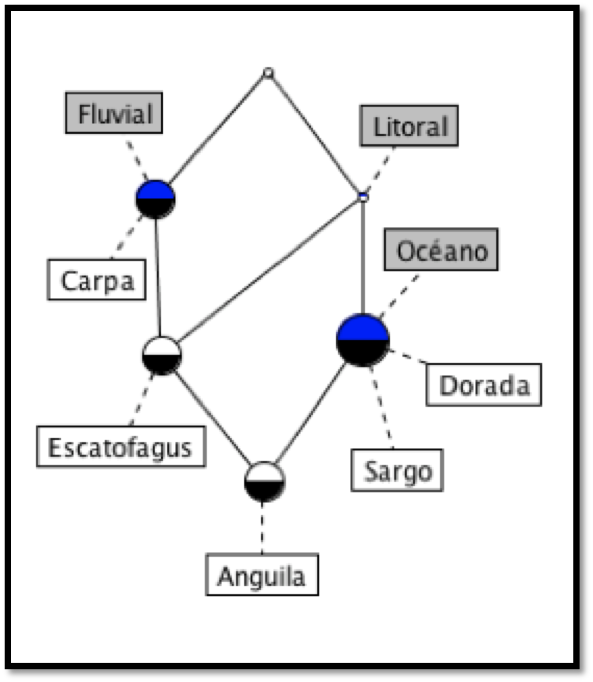
\includegraphics[scale=0.75]{img/2/reticulo}
\caption{Retículo de Conceptos
\label{fig:reticulo}}
\end{figure}



\section{Bases Stem.}

\begin{defi}
Para un contexto ${\cal K}:=(G,M,I)$, Una {\bf implicación} entre atributos es una expresión de la forma $Y_1 \rightarrow{Y_2}$, dónde $Y_1, Y_2 \subseteq M$; es decir, son subconjuntos de atributos.
\end{defi}

El objetivo es obtener un conjunto de relaciones entre los atributos, para que, usando operaciones lógicas, se pueda trabajar con el contexto dado.

A continuación se definen una serie de características sobre las implicaciones. Sea ${\cal L}$ un conjunto de implicaciones; se tiene:
\begin{enumerate}
	\item ${\cal L} \ \models Y \rightarrow{Z}$ ($Y \rightarrow{Z}$ es {\bf consecuencia} de ${\cal L}$) si para todo $T \subseteq M$, si $T$ respeta ${\cal L}$ entonces $T$ respeta $Y \rightarrow{Z}$.
	\item ${\cal L}$ es {\bf cerrada} si contiene a toda implicación $Y \rightarrow{Z}$ que es consecuencia de ${\cal L}$.
	\item ${\cal L}$ es {\bf completo} si toda implicación válida en $(G,M,I)$ es consecuencia de ${\cal L}$:
	\begin{center}
		$(G,M,I) \models Y \rightarrow{Z}\ \ \Longrightarrow{\ \  {\cal L} \ \models Y \rightarrow{Z} }$
	\end{center}
	\item ${\cal L}$ es {\bf no redundante} si ninguna implicación de ${\cal L}$ es consecuencia del resto:
	\begin{center}
		$Y \rightarrow{Z} \in{{\cal L}}\ \ \Longrightarrow{\ \  {\cal L} \backslash \{ Y \rightarrow{Z}\} \not\models Y \rightarrow{Z} }$
	\end{center}
\end{enumerate}

\begin{defi}
	Se define como {\bf Base Stem} al conjunto {\bf completo} e {\bf irredundante} de implicaciones de un contexto ${\cal K}:=(G,M,I)$.
\end{defi}

El problema se reduce, pues, a obtener una Base Stem para un contexto dado. Para ello, se hará uso del cálculo implicacional basado en las Reglas de Amstrong:

\begin{center}
\begin{minipage}[t]{0.3\linewidth} \centering
	$R_1: \frac{}{X\rightarrow{X}}$
\end{minipage}
%\hspace{0.5cm}
\begin{minipage}[t]{0.3\linewidth} \centering
	$R_2: \frac{X\rightarrow{Y}}{X \cup Z \rightarrow{Y}}$
\end{minipage}
%\hspace{0.5cm}
\begin{minipage}[t]{0.3\linewidth} \centering
	$R_3: \frac{X\rightarrow{Y}, Y \cup Z \rightarrow{W}}{X \cup Z \rightarrow{W}}$
\end{minipage}
\end{center}

Con este conjunto de reglas, se puede obtener el siguiente cálculo lógico:

\begin{center}
	${\cal L} \vdash L \Longleftrightarrow{L}$ se prueba mediante las reglas de Amstrong a partir de ${\cal L}$.
\end{center}

\begin{teo}
	Si ${\cal L}$ es un conjunto Stem para un contexto formal ${\cal K}$, entonces ${\cal L}$ proporciona una teoría implicacionalmente completa para ese modelo; es decir:
	\begin{center}
	$ {\cal L} \vdash L \Longrightarrow{ {\cal K} \models L }$
	\end{center}
\end{teo}

\begin{defi}
	$P \subseteq M$ es una {\bf pseudointención} de un contexto ${\cal K}:=(G,M,I)$ si se verifica que:
	\begin{itemize}
		\item $P \neq P''$
		\item Para toda pseudointención $Q \subset P$, se verifica que $Q'' \subseteq P$.
	\end{itemize}
\end{defi}

\begin{teo}
	El conjunto $\{P \rightarrow {P''} | P \mbox{ es pseudointención}\}$ es una Base Stem del Contexto. \\
	En la práctica, únicamente se toman las implicaciones $P \rightarrow {(P''-P)}$, ya que $P \rightarrow {P}$ siempre es válido.
\end{teo}

A cada pseudointención podemos añadirle un atributo de {\bf soporte}, que indica el número de objetos que cumplen esta implicación. Este soporte será un entero mayor o igual a cero.

Veamos en nuestro ejemplo, la traza del algoritmo seguido para calcular las distintas pseudointenciones del contexto. Dado que la definición de pseudointención es recursiva, iniciaremos con el conjunto vacío, e iremos recorriendo los subconjuntos de menor a mayor tamaño. De esta forma, las pseudointenciones calculadas previamente nos pueden ayudar a descartar otras pseudointenciones en el proceso. Por mejorar la visibilidad, únicamente se expresarán las iniciales de los atributos y de los objetos.

\begin{itemize}
	\item $\emptyset_M = G = \emptyset_M$; por tanto, NO.
	\item $\{f\}'' = \{c,e,a\}' = \{f\}$; por tanto, NO.
	\item $\{l\}'' = \{e,s,d,a\}' = \{l\}$; por tanto, NO.
	\item $\{o\}'' = \{s,d,a\}' = \{l,o\}$; por tanto, SÍ.
	\item $\{f,l\}'' = \{e,a\}' = \{f,l\}$; por tanto, NO.
	\item $\{f,o\}'' = \{a\}' = \{f,l,o\}$; sin embargo se tiene que $\{o\}\subset\{f,o\}$, \\ y $\{o\}'' = \{l,o\} \not\subseteq \{f,o\}$; por tanto NO.
	\item $\{l,o\}'' = \{s,d,a\}' = \{l,o\}$; por tanto NO.
	\item $\{f,l,o\}'' = \{a\}' = \{f,l,o\}$; por tanto, NO.
\end{itemize}

Por tanto, la Base Stem obtenida (simplificando las implicaciones) en el ejemplo que hemos seguido a lo largo de todo el capítulo, es:
\begin{itemize}
	\item $(\{oceanico\} \rightarrow {\{litoral\}})$, con soporte 3 (puesto que 3 objetos la cumplen).
\end{itemize}


   % 
\chapter{Extracción de Conocimiento en Sistemas de Etiquetado.}\label{cap:capitulo3}

En este capítulo vamos a ver algunas características de los Sistemas de Etiquetado (SE), se enlazarán estas características con los elementos formales que se han visto en el capítulo anterior; y finalmente se comentarán las relaciones entre usuarios desde el punto de vista del Análisis Formal de Conceptos (AFC).

\section{Estructura de los Sistemas de Etiquetado.}

Existen multitud de Sistemas de Etiquetado. En \cite{smith} se citan un gran número de ejemplos, y se explica las diferentes estructuras de cada uno de ellos.

En este trabajo, vamos a centrarnos en Delicious (\cite{delicious}) como Sistema de Etiquetado, y en la folksonomía que el sistema ofrece a partir de la actuación colaborativa de los usuarios. Tomaremos la definición de folksonomía dada en \cite{jaschke}:

\begin{defi}
Una {\bf folksonomía} es una tupla ${\cal F} := (U,E,R,Y)$, dónde:
\begin{itemize}
	\item $U$, $E$ y $R$ son conjuntos finitos, cuyos elementos son, respectivamente, los usuarios, etiquetas y recursos del sistema. En sistemas como Delicious, los recursos son URLs y las etiquetas son campos de texto.
	\item $Y$ es una relación ternaria entre ellos; es decir, $Y  \subseteq \{ U \times{E \times{R}}\}$, cuyos elementos se conocen como etiquetaciones.
\end{itemize}
\end{defi}

Existe un consenso en cuanto a la estructura de este tipo de sistemas, como se puede ver en diferentes definiciones (como en \cite{golder} o \cite{yeung}).

Como se ha comentado en capítulos anteriores, el sistema se va creando gracias a las aportaciones colaborativas de todos los usuarios, que, unido a las características del sistema (no jerárquico y no exclusivo), potencian su popularidad, lo que a su vez genera nuevos usuarios y nuevas aportaciones; el conjunto de datos está en continuo crecimiento. Sin embargo, el problema de heterogeneidad semántica en cuanto a la etiquetación que cada usuario realiza hace que no se produzca un consenso por parte de todos ellos. Por ello, emergen ciertos métodos de resolución de estos conflictos para un posterior procesado de todo el volumen de datos que el sistema posee, que puede llegar a ser muy útil en algunos casos.

En \cite{golder}, se presentan pruebas empíricas sobre la actividad de los usuarios, expresadas en el número de etiquetas que cada usuario usa, la tasa de crecimiento de cada etiqueta, así como el uso de ciertas URLs y la etiquetación de las mismas.

En cuanto al número de etiquetas, existen comportamientos diferentes. Inicialmente, el número de etiquetas por usuario crece en todos los casos. Sin embargo, llegado un punto, existen usuarios que siguen añadiendo nuevas etiquetas, por lo que este número sigue creciendo; mientras otros estabilizan el número de etiquetas que usan, y todas las etiquetaciones que realizan, las hacen con algunas de las etiquetas ya utilizadas.

Por norma general, el uso de una etiqueta va creciendo a lo largo del tiempo, ya que siempre aparecen nuevos usuarios que comienzan a usar esta etiqueta. En el caso de los enlaces es diferente, ya que normalmente emerge un comportamiento en el cual se produce un momento puntual en el cual se producen muchas etiquetaciones de ese enlace de forma masiva, y luego vuelve a descender para seguir unas tasas más pequeñas. Este crecimiento puntual se suele producir o bien al inicio del ciclo de vida de dicho enlace en el sistema, o bien una vez que ha transcurrido un largo período.




\section{Contextos y Conceptos Formales.}

El estudios de los Sistemas de Etiquetado desde el punto de vista formal ha sido un campo de trabajo muy concurrido en los últimos tiempos, y podemos encontrar una gran variedad de propuestas en diversas publicaciones: en \cite{alonso} se propone un método de extensión de atributos; en \cite{yeung} se ofrece un método para minimizar los efectos de hetereogenidad semántica; en \cite{van} se propone un método para convertir en ontologías estas folkonomías; etc...

En el capítulo~\ref{cap:capitulo2} se han introducido las características de los Contextos formales. Estos contextos están formado por un conjunto $G$ de objetos, un conjunto $M$ de atributos, y una relación binaria $I$ entre ambos.

Existe una analogía clara entre estos Contextos formales y los Sistemas de Etiquetado. De hecho, todo Sistema de Etiquetado puede transformarse en un conjunto de Contextos formales. Formalicémoslo:

\begin{teo}
Toda folksonomía ${\cal F} := (U,E,R,Y)$ es transformable en un conjunto de Contextos formales ${\cal K}_i := (G_i, M_i, I_i)$ mediante una función $\gga$, de forma que:
\begin{center}
	$\gga({\cal F}) = \bigcup \limits_{k=1}^{size(U)} {{\cal K}_{\mbox{\scriptsize \emph{k}}}}$
\end{center}

La demostración es trivial estableciendo que $G_i \subseteq R$, $M_i \subseteq E$ e $I_i \subseteq (R \times{E})$. Concretamente está relación binaria $I_i$ se consigue fijando el valor de cada usuario en la relación ternaria $Y$; ésta es la razón por la que se obtienen $size(U)$ contextos diferentes. Los conjuntos $G_i$ y $M_i$ están formados por los objetos y atributos que participan en la relación binaria obtenida anteriormente.
\end{teo}


El teorema anterior nos permite transformar un Sistema de Etiquetado (o un subconjunto completo de éstos) en un conjunto de Contextos Formales. En total se obtienen tantos contextos como usuarios forman parte del Sistema de Etiquetado.

En el caso concreto de este trabajo, cada contexto estará formado por un conjunto de enlaces (objetos) y un conjunto de atributos (atributos), que es precisamente lo que cada usuario aporta de forma colaborativa al sistema de Delicious.

Para cada uno de los contextos anteriores, se puede calcular fácilmente los Retículos de Conceptos que representan el contexto, y las Bases Stem asociadas a éstos.








\section{Relaciones entre usuarios.}

En la sección anterior se ha visto cómo extraer un conjunto de Contextos (formales) de un Sistema de Etiquetado. Cada uno de estos contextos representa el conocimiento de cada usuario dentro del sistema. Es posible establecer una serie de relaciones entre los usuarios, o más bien, entre los contextos de cada uno de ellos. Las más importantes, que son las que utilizaremos en este trabajo, son: Lenguaje común y Conjunto de Objetos comunes.

\begin{itemize}
	\item {\bf Lenguaje común}: Dados dos usuarios y los contextos formales de cada uno de ellos, el lenguaje común es el conjunto de atributos que ambos usuarios tienen. Sean $M_1$ y  $M_2$ los conjuntos de atributos de cada usuario respectivamente; el lenguaje común $\cal{L}$ es precisamente la intesección de estos dos conjuntos:
\begin{center}
	${\cal L} = M_1 \cap M_2$
\end{center}

	\item {\bf Conjunto de Objetos comunes}: Dados dos usuarios y los contextos formales de cada uno de ellos, el conjunto de Objetos comunes es el conjunto de objetos que ambos usuarios tienen. Sean $G_1$ y $G_2$ los conjuntos de objetos de cada usuario respectivamente; el conjunto de objetos comunes ${\cal O}$ es precisamente la intersección de estos dos conjuntos:
\begin{center}
	${\cal O} = G_1 \cap G_2$
\end{center}
\end{itemize}

Además de las dos relaciones anteriores, se pueden establecer otro tipo de relaciones entre usuarios. Se pueden establecer restricciones en las relaciones anteriores para crear nuevas relaciones. Por ejemplo, se puede establecer un lenguaje común reducido entre dos usuarios escogiendo sólo aquellos atributos que, además de pertenecer al lenguaje común, son parte de alguna etiquetación en el mismo enlace para ambos usuarios. Es obvio que este nuevo lenguaje común reducido es bastante más pequeño que aquel en el que no se impone ninguna restricción. Igualmente, se puede crear un conjunto de objetos comunes reducido escogiendo únicamente los enlaces que, además de pertenecer al conjunto inicial de objetos comunes, están etiquetados con una misma etiqueta por ambos usuarios. Igualmente, este último conjunto es mucho más pequeño que el inicial.

Por último, hay que indicar que se pueden establecer tantas relaciones como criterios se quieran inventar. Sin embargo, en este trabajo sólo hemos utilizado las dos anteriores: el Lenguaje común servirá para crear contextos reducidos en los que sólo existan objetos etiquetados con etiquetas pertenecientes a este lenguaje, previo a la conciliación del conocimiento de ambos usuarios; el conjunto de objetos comunes servirá para decidir que pares de usuarios deben realizar conciliación y cuáles no, esto se decidirá en función del tamaño de este conjunto. En este trabajo, únicamente se producirá conciliación entre dos usuarios cuando compartan 3 objetos o más; es decir, cuando esté conjunto de objetos comunes esté formado por 3 o más objetos. 

   % 
\begin{thebibliography}{99}

\addcontentsline{toc}{chapter}{Bibliografía.}

\bibitem{alonso} Alonso-Jiménez, J.A., Aranda-Corral, G.A., Borrego-Díaz, J., Fernández-Lebrón,
M.M., Hidalgo-Doblado, M.J. (2008). Extending Attribute Exploration by Means of Boolean Derivatives. In: Proc. 6th Int. Conf. on Concept Lattices and Their Applications. CEUR Workshops Proc., p. 433. 

\bibitem{algoritmo} Aranda-Corral, G.A., Borrego-Díaz, J. (2010). Reconciling Knowledge in Social Tagging Web Services. Lecture Notes in Computer Science, 6077(1), 101-121.

\bibitem{mowento} Aranda-Corral, G.A., Borrego-Díaz, J., Gómez-Marín, F. (2009). Toward Semantic Mobile Web 2.0 through Multiagent Systems. In: Håkansson, A., Nguyen, N.T., Hartung, 
R.L., Howlett, R.J., Jain, L.C. (eds.) KES-AMSTA 2009. LNCS, vol. 5559, pp. 400–409. Springer, Heidelberg.

\bibitem{blondel} Blondel, V.D., Guillaume, J.L., Lambiotte, R., Lefebvre, E. (2008). Fast unfolding of communities in large networks. Journal of Statistical Mechanics: Theory and Experiment, Vol. 2008, No. 10.

\bibitem{brooks} Brooks, C.H., Montanez, N. (2006). Improved annotation of the blogosphere via autotagging and hierarchical clustering. In WWW 06. Proceedings of the 15$^{th}$ international conference on World Wide Web, (pp.625-632.). New York: ACM Press.  

\bibitem{afc} Ganter, B., Wille, R. (1999). Formal Concept Analysis - Mathematical Foundations. Springer, Heidelberg.

\bibitem{golder} Golder, S., Huberman, B.A. (2006). The structure of collaborative tagging systems. Journal of Information Science 32(2), 98-208.

\bibitem{gruber} Gruber, T. (2007). Ontology of Folksonomy: A Mash-up of Apples and Oranges. Int'l. Journal on Semantic Web \& Information Systems 3(2).

\bibitem{halpin} Halpin, H., Valentin R., and Hana S. (2006). The dynamics and semantics of collaborative tagging. Proceedings of the 1$^{st}$ Semantic Authoring and Annotation Workshop (SAAW06). 

\bibitem{jaschke} Jäschke, R., Hotho, A., Schmitz, C., Ganter, B., Stumme, G. (2008). Discovering shared conceptualizations in folksonomies. Journal of Web Semantics 6(1), 38–53.

\bibitem{kim} Kim, H.-L., Scerri, S., Brslin, J., Decker, S., Kim, H.-G. (2008). The state of the art in tag ontologies: A semantic model for tagging and folksonomies. In: International Conference on Dublin Core and Metadata Applications, Berlin, Germany.

\bibitem{knerr} Knerr, T. (2006). Tagging ontology-towards a common ontology for folksonomies. \url{http:// tagont.googlecode.com/files/TagOntPaper.pdf}.

\bibitem{mathes} Mathes, A. (2004). Folksonomies - Cooperative Classification and Communication Through Shared Metadata. \url{http://www.adammathes.com/academic/computer-mediated-communication/folksonomies.html}

\bibitem{mika} Mika, P. (2005). Ontologies Are Us: A unified model of social networks and semantics. Proceedings of the 4$^{th}$ International Semantic Web Conference, ISWC 2005, Galway, Ireland, (pp. 522-536). Berlin, Heidelberg: Springer.  

\bibitem{rowley} Rowley, J. (1995). Organizing Knowledge. 2$^{\mbox{\scriptsize nd}}$ Ed. Brookfield, VT: Gower.

\bibitem{shirky} Shirky, C. (2005). Ontology is Overrated: Categories, Links and Tags. \url{http://www.shirky.com/writtings/ontology_overrated.html}

\bibitem{smith} Smith, G. (2007). Tagging: People-Powered Medatada for the Social Web. First. New Riders Publishing, Indianapolis.

\bibitem{tanaka} Tanaka, J.W., Taylor, M. (1991) . Object categories and expertise: Is the basic level in the eye of the beholder? Cognitive Psychology 23(3), 457–482.

\bibitem{van} Van Damme, C., Hepp, M., Siorpaes, K. (2007). FolksOntology: An Integrated Approach for Turning Folksonomies into Ontologies. In: ESWC 2007 workshop Bridging the Gap between Semantic Web and Web 2.0, May 2007, pp. 57–70.

\bibitem{weick} Weick, K.E., Sutcliffe, K.M., Obstfeld, D. (2005). Organizing and the Process of Sense\-making. Organization Science 16(4), 409–421.

\bibitem{yeung} Yeung, C.M.A., Gibbins, N., Shadbolt, N. (2009). Contextualising Tags in Collaborative Tagging Systems. In: Proceedings of the 20th ACM Conference on Hypertext and 
Hypermedia.


\bibitem{conexp} ConExp: \url{http://conexp.sourceforge.net/}

\bibitem{delicious} Delicious: \url{http://www.delicious.com/}

\bibitem{dot} Notación DOT: \url{http://www.graphviz.org/Documentation.php}

\bibitem{fipa} FIPA (Foundation for Intelligent Physical Agents): \url{http://www.fipa.org/}

\bibitem{gephi} Gephi: \url{http://gephi.org/}

\bibitem{jade} JADE (Java Agent Development Framework): \url{http://jade.tilab.com/}

\end{thebibliography}









%%  Apendices
%%%%%%%%%%%%%%%%%%%%%%%%%%%%%%%%%%%%%%%%%%%%%%%%%%%%%%%%%%%%%%%%%%%%%%

%\appendix
%\include{apendice}  % Puedo poner la ontología OSMV y la arquitectura de OW

%%  Bibliografia
%%%%%%%%%%%%%%%%%%%%%%%%%%%%%%%%%%%%%%%%%%%%%%%%%%%%%%%%%%%%%%%%%%%%%%
\newpage
\addcontentsline{toc}{chapter}{Bibliografía}
\bibliographystyle{alpha}
\bibliography{biblio/bibliografia.tex}

\end{document}

